\section{Adaptive Protection}
\label{amsstrategy}
In the previous section, we have shown how we can model a security attack as a Markov game between the attacker and the defender. From the system architect, one important question is how the system should choose its defending strategy in order to minimize the amount of damage caused by the attacker. A conventional approach in the game theory is computing a \textit{Nash equilibrium} (NE) strategy: that is, both the attacker and the defender play a strategy that would maximize the payoffs for both of them \cite{law2012security, ma2013markov}. The rationale for adopting the NE solution is that neither the attacker nor the defender can do better by choosing a different strategy.

However, in practice, choosing a NE strategy is not necessarily optimal for the defender, since it depends on a number of assumptions that might not hold. First, computing a NE relies on a perfect knowledge of the system; however, in reality, the attacker might not have the capability to collect enough information to construct an accurate model of a smart grid. Second, since the attackers are humans, it is likely that they would launch attacks based on their intuition or past experience, which might be different from the NE strategy. Lastly, if there are multiple equilibria, the players may not pick the same matching strategy.

Instead, an effective defending strategy should be \textit{adaptive}, i.e., it should be able to learn the attacker's strategy and dynamically compute the \textit{best response} strategy to counter the attacking strategy. However, assuming that the attacker may change its strategy arbitrarily is neither useful nor practical. Therefore, to make our technique feasible, we assume that the attacker's strategy is \textit{stationary} (i.e., the probability of choosing each action is unchanged under the same state)\footnote{We allow the attacker to change its strategy to another stationary strategy during the game.}.

An effective defending strategy must satisfy the following two desirable properties \cite{bowling2001convergence}.

\begin{description}
\item[Rationality] A \emph{rational} defending strategy must always learn to play the best response strategy given that the attacker is adopting a stationary attacking strategy. Satisfying this property guarantees that the cost to the system can be minimized as long as the attacker's strategy is stationary. Note that a NE strategy is a special case of stationary strategy.

\item[Convergence] The defending strategy must always converge to a stationary strategy under self-play.  This property takes into consideration the possibility that the attacker might be as intelligent as the defender and employ the same adaptive strategy as the defender. We can see that under self-play, if both rationality and convergence properties are satisfied, the defender and attacker will eventually converge to a NE strategy. This means that the maximum cost to the system can be bounded to the cost when the attacker adopts a NE strategy, even when the attacker is as intelligent as the defender.
\end{description}

\subsection{AMS: Adaptive Markov Strategy}

In this section, we propose an algorithm for computing an \underline{a}daptive \underline{M}arkov \underline{s}trategy (AMS) for defending a system against security attacks. Our algorithm is based on the AWESOME algorithm~\cite{conitzer2007awesome}, which computes adaptive defending strategies for repeated games only (i.e., a special case of Markov games where the system has exactly one state); we extend AWESOME to Markov games where the system may have any finite number of states.  

Before introducing the AMS algorithm in details, we need to explain a few terms first. First, to determine whether the attacker is employing the NE or any other stationary strategies, we define the \emph{distance} between two strategies to compare whether they are the same or not. 

\begin{definition}
The \emph{distance} $Distance(\phi_1, \phi_2)$ between two stationary strategy $\phi_1$ and $\phi_2$ is: 
\begin{equation}
Distance(\phi_1, \phi_2) = \max|\phi_1(s,a) - \phi_2(s,a)|, \forall a\in A_s, s\in S
\end{equation}
where $A_s$ is the action space at state $s$ and $S$ is the state space, and $\phi_1(s,a)$ and $\phi_2(s,a)$ is the probability that action $a$ is played at state $s$ for strategy $\phi_1$ and $\phi_2$ respectively.
\end{definition}

Second, given two strategies $\phi_1$ and $\phi_2$, we define the value $V(s, \phi_1, \phi_2)$ of playing strategy $\phi_1$ against strategy $\phi_2$ under state $s$, which is defined as the sum of the discounted expected payoff obtained over infinite number of interactions.
\begin{definition}
\label{valueofstate}
The value $V(s, \phi_1, \phi_2)$ of playing strategy $\phi_1$ against strategy $\phi_2$ under state $s$ is defined as follows, 
\begin{equation}
\begin{split}
V(s, \phi_1, \phi_2) = &R(s, \phi_1(s), \phi_2(s)) +\\& \delta\sum_{s\in S} Pr(\phi_1(s), \phi_2(s), s, s^\prime)V(s^\prime, \phi_1, \phi_2)
\end{split}
\end{equation}
\end{definition}
where $\delta$ is the discounting factor reflecting the relative importance of future payoffs and $Pr(\phi_1(s), \phi_2(s), s, s^\prime)$ is the probability that the system state transits from $s$ to $s^\prime$ given that the players choose actions $\phi_1(s)$ and $\phi_2(s)$ respectively. We can construct one equation for V-value of each state $s\in S$ following Definition \ref{valueofstate}, and thus the value of each state can be calculated by solving the system of $|S|$ linear equations using different techniques such as iterative methods \cite{eisenstat1983variational}.

The AMS algorithm (Algorithm \ref{AMS}) takes place over consecutive \textit{periods} (where each period is some number of round)\footnote{Each round of attacker-defender interaction might take a few minutes in the smart-grid system.}. Initially, the AMS begins by playing the precomputed NE strategy\footnote{We only need to compute the minmax strategy instead since for a zero-sum Markov game, the minmax/maxmin strategy for each player is equivalent with its corresponding NE strategy \cite{sigaud2013markov}. Generalized value iteration algorithm \cite{sigaud2013markov} can be used to compute the minmax strategy efficiently and we omit the details due to space limitation.} for the initial period $N^0$ (Line 5) and estimates the strategy of the attacker based on the actions taken in this period (Line 7 to 10). If the \emph{distance} between the estimated strategy $h_a^{curr}$ and the NE strategy $\pi_a^*$ of the attacker is larger than the given threshold (line 13), the attacker is considered playing a non-NE strategy, and a random strategy is chosen as the defense strategy for the next period (Line 17). 

\begin{algorithm}[t]\small
\caption{Description of AMS}
\label{AMS}
\begin{algorithmic}[1]
\STATE Compute NE strategy ($\pi^*_i, \forall i\in\{d,a\}$)
\REPEAT 
\STATE Initialize $h_a^{prev}$, $h_a^{curr}$ to nil
\STATE $s = s_0$, $\beta = false$, $t = 0$
\STATE Set defender strategy $\phi_d$ as NE strategy ($\phi_d = \pi_d^*$)
\WHILE{true}
\FOR{$r$ : 0 \TO  $N^t$}
\STATE Play($\phi_d(s)$)
\STATE Update($h_a^{curr}$)
\ENDFOR
\STATE $h_a^{prev} = h_a^{curr}$
\STATE $t$ := $t + 1$

     \IF{Distance($h_a^{curr}$, $\pi_a^*$) > $\epsilon^t_e$}
     \STATE  \textbf{break}
      \ENDIF
\ENDWHILE

\STATE $\phi_d$ = RandomStrategy()
\WHILE{true}
\FOR{$r$ : 0 \TO  $N^t$}
\STATE Play($\phi_d(s)$)
\STATE Update($h_a^{curr}, h_a^{prev}$)
\ENDFOR
\STATE $t$ := $t + 1$

  \IF{$\beta$ = true}
     \IF{Distance($h_a^{curr}$, $h_a^{prev}$) > $\epsilon^t_s$}
        \STATE \textbf{break}
      \ENDIF
  \ENDIF
  \STATE $h_a^{prev} = h_a^{curr}$
   \STATE $\beta := true$
   \STATE $\phi_d^\prime$ := BestResponseStrategy($h_a^{curr}$)
   \IF{$V(s,\phi_d^\prime, h_a^{curr}) > V(s,\phi_d, h_a^{curr}) + 2|A|^{|S|}\epsilon^{t+1}_s\mu$, $\forall s \in S$}
       \STATE $\phi_d = \phi_d^\prime$
   \ENDIF
\ENDWHILE
\UNTIL{}
\end{algorithmic}
\end{algorithm}

At the end of the next period, AMS computes the best response strategy $\phi_d^\prime$  against the current estimated strategy $h_a^{curr}$ of the attacker based on the last period's interaction (Line 31).\footnote{Generalized value iteration algorithm can be adopted here to compute the best response strategy in a Markov game \cite{sigaud2013markov}, and we skip the details due to space limitation.} If for every state $s\in S$, the difference between the V-value of $\phi_d^\prime$ against the $h_a^{curr}$ and that of $\phi_d$ is larger than the given threshold $2|A|^{|S|}\epsilon^{t+1}_s\mu$ (where $|A|^{|S|}$ represents the total number of pure strategies of the Markov game and $\mu$ is the payoff difference between the AMS player's best and worse outcomes), the current defending strategy $\phi_d$ is replaced by a more optimal strategy $\phi_d^\prime$ (Line 32-34).


\begin{figure*}[t]
\setlength{\belowcaptionskip}{-10pt}
\centering
 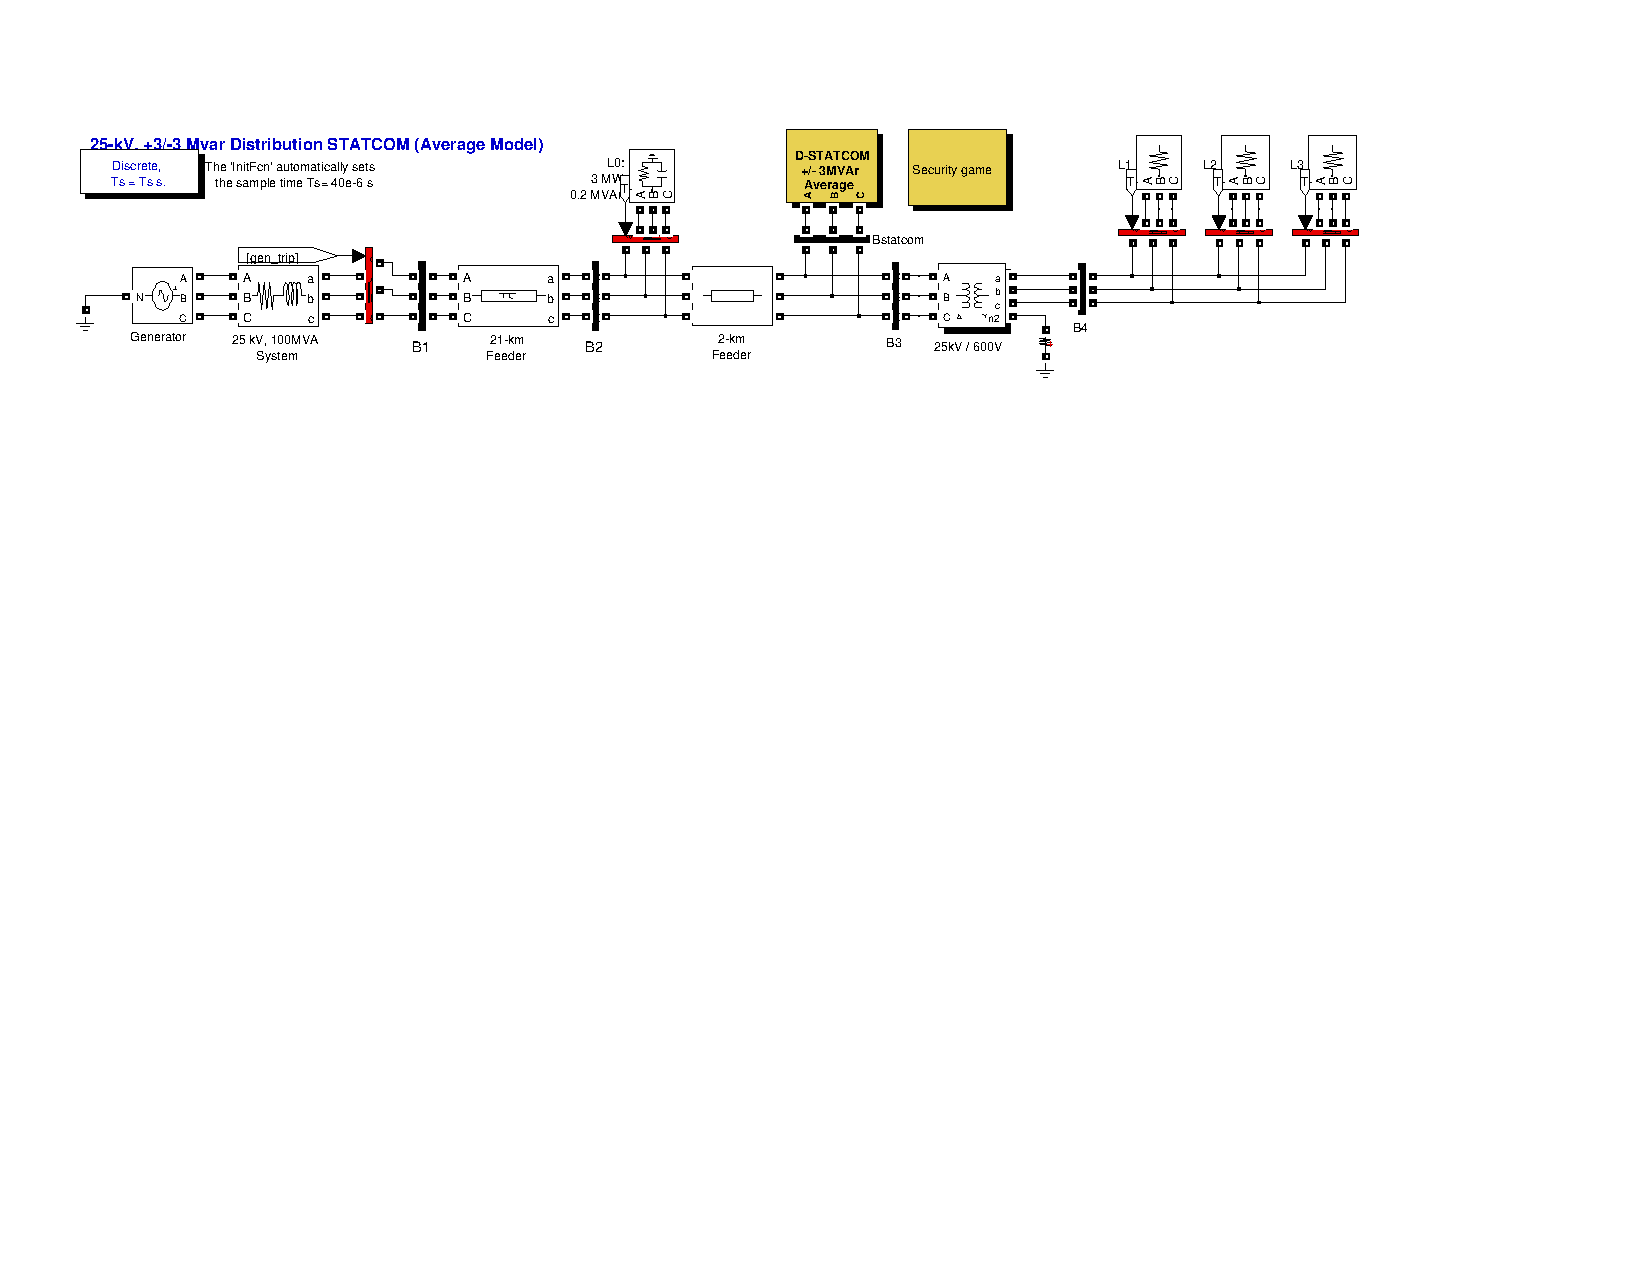
\includegraphics[width=0.95\textwidth]{example}
\caption{\scriptsize{An example distribution system with 1 generator and 4 buses \cite{law2012security}, originally from the D-STATCOM model in SimPowerSystems~\cite{simpowersystems}.}}
 \label{fig:example}
\end{figure*}

At the end of each following period, AMS compares the estimated strategy $h_a^{curr}$ and $h_a^{prev}$ of the attacker in the last and preceding periods (Line 25). If the distance between these two is larger than the given threshold $\epsilon_s^t$, it indicates that the opponent is not playing according to the estimated strategy $h_a^{prev}$, and the AMS will restart by breaking from the second while loop (Line 26). Otherwise, the AMS computes a best response strategy $\phi_d^\prime$ based on the last period's interaction, and employs $\phi_d^\prime$ as its strategy if it is more optimal than $\phi_d$ (Line 31-34). This process repeats as indicated by the outer \emph{Repeat} loop. 

The remaining question is how the set of parameters of the AMS algorithm should be adjusted, described as follows.

\begin{definition}
A schedule of adjusting the parameters \\$\{\epsilon_e^t, \epsilon_s^t, N^t\}$ is valid if
\begin{itemize}
\item $\epsilon_e^t, \epsilon_s^t$ are decreased monotonically and converge to zero eventually.
\item the value of $N^t$ is increased monotonically to infinity.
\item $\Pi_{t\in\{1,2,\ldots\}}(1 - A_S\frac{1}{N^t(\epsilon_s^{t+1})^2}) > 0$, where $A_S$ is the total number of actions of the defender summed over all states.
\end{itemize}
\end{definition}

\subsection{Properties of the AMS}

As previously mentioned, an effective defending strategy must satisfy two desirable properties: rationality and convergence. It can be theoretically proved that the AMS satisfies both properties, which are formalized as the following two theorems: 

\begin{theorem}
\label{rationality}
Given a valid schedule of adjusting the parameters, if the attacker employs a stationary attacking strategy, the defender adopting AMS eventually converges to a best response to the attacker's strategy with probability one.
\begin{proof}
We only provide a sketch of the proof here due to limited space. This theorem can be proved by dividing it into two parts. First, we prove that with non-zero probability, the AMS will never restart. We can show that the joint probability that the AMS will not restart for every period $t$ is greater than zero based on the triangle inequality and Chevyshev's inequality theorem. 

Second, we prove that the probability that the AMS never restarts and does not converge to a best response strategy against the attacker is 0 by continuity and Chevyshev's inequality theorem.  By proving both parts, we can conclude that the AMS will converge to a best response strategy against the attacker with probability 1.
\end{proof}
\end{theorem}

\begin{theorem}
\label{convergence}
Given a valid schedule, if both the defender and attacker employ the AMS, they eventually converge to a NE with probability one.
\begin{proof}
This theorem can be proved in a similar way to Theorem \ref{rationality}, and we omit the details due to limited space.
\end{proof}
\end{theorem}